In task 4 we want to take the vehicle dynamics linearized about the (optimal) trajectory $(x_{opt}, u_{opt})$ computed in
Task 2 and then exploit an MPC algorithm to track this reference trajectory.

\section{Model Predictive Control}

The goal of Model predictive Control (MPC) is to control a system via a stabilizing controller that minimizes a certain cost function, enforces some constraint for all t and works online. This is implemented by solving an optimal control problem at each sampling time and applying the first optimal input: 

For each t: 
\begin{itemize}
    \item Measure the current state $x_t$
    \item Compute the optimal trajectory $x^{*}_{t|t},..., x^{*}_{t+T|t}, u^{*}_{t|t}, ..., u^{*}_{t+T-1|t}$ with initial condition $x_t$
    \item Apply the first control input $u^{*}_{t|t}$
    \item Measure $x_{t+1}$ and repeat
\end{itemize}

\begin{figure}[htp]
\centering
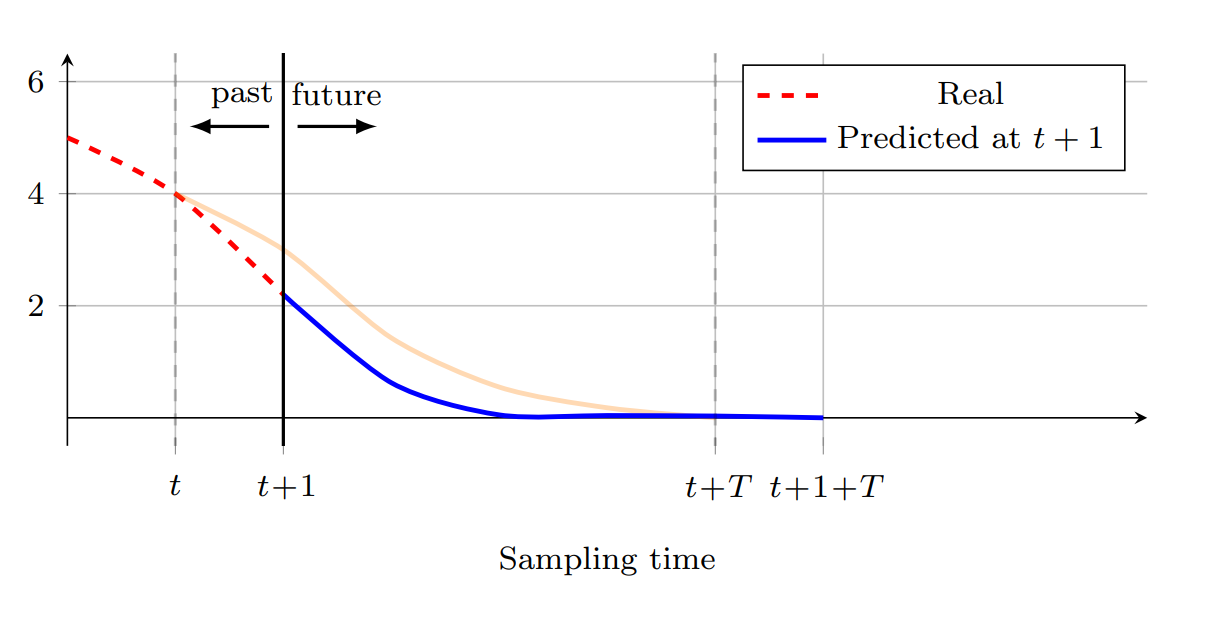
\includegraphics[width=0.5\textwidth]{pictures/MPC}
\caption{Model Predictive Control}
\label{fig:MPC}
\end{figure}


\subsection{The optimal control problem to be solved at each t}

At each time instant we want to solve

\begin{align*}
\min_{\substack{x_t,...,x_{t+T} \\ u_t,...,u_{t+T-1}}} &\sum_{\tau=t}^{t+T-1} l_\tau (x_\tau, u_\tau) + l_{t+T}(x_{t+T})
\end{align*}

\begin{align*} subject \quad to \qquad 
 x_{\tau+1} = f(x_\tau, u_\tau) \qquad \forall \tau = t, ..., t+T-1 \\ 
 x_{\tau} \in \textit{X}, u_{\tau} \in \textit{U} \qquad \forall \tau = t, ..., t+T \qquad\\
 x_t = x^{meas}_t \qquad \qquad \qquad \qquad \qquad \qquad 
\end{align*}

where 
\begin{itemize}
    \item $x_{\tau + 1} = f(x_\tau, u_\tau)$ is the so-called prediction model
    \item $x^{meas}_t$ is the state (of the real system) measured at t
\end{itemize}

\subsection{The Linear Quadratic Case}

In our case, the dynamics is linear because we linearized it about the optimal trajectory $(x_{opt}, u_{opt})$ computed in task 2. Therefore we can consider the MPC case where the dynamics is linear and the cost quadratic: 

At each time t with initial measured state $x_t^{meas}$ we want to solve the LQ problem 

\begin{align*}
\min_{\substack{x_t,...,x_{t+T} \\ u_t,...,u_{t+T-1}}} &\sum_{\tau=t}^{t+T-1} x_\tau^T Q_\tau x_\tau + u_\tau^T R_\tau u_\tau + x_{t+T}^T Q_T x_{t+T}
\end{align*}

\begin{align*} subject \quad to \qquad 
 x_{\tau+1} = A_\tau x_\tau + B_\tau u_\tau \qquad \forall \tau = t, ..., t+T-1 \\ 
 x_t = x^{meas}_t \qquad \qquad \qquad \qquad \qquad \qquad \qquad \quad 
\end{align*}

where  
\begin{itemize}
    \item T is the prediction horizon
    \item $x_{\tau} \in \mathbb{R}^n$ and $u_{\tau} \in \mathbb{R}^m$
    \item $A_{\tau} \in \mathbb{R}^{nxn}$ and $B_{\tau} \in \mathbb{R}^{nxm}$ is the prediction model 
    \item $Q_{\tau} \in \mathbb{R}^{nxn}$ and $Q_{\tau} = Q_{\tau}^T \geq 0 \forall \tau$  
    \item $R_{\tau} \in \mathbb{R}^{mxm}$ and $R_{\tau} = R_{\tau}^T > 0 \forall \tau$ 
    \item $Q_{T} \in \mathbb{R}^{nxn}$ and $Q_{T} = Q_{T}^T \geq 0 $ 
    
\end{itemize}

\section{Tracking of $(x_{opt}, u_{opt})$}
Since we want to track the optimal trajectory throught Model Predictive Control, the cost function that we are interested in minimizing is the one in which $x_\tau$ and $u_\tau$ are the errors between the predicted trajectory ($x^{mpc}$, $u^{mpc}$) and the optimal one ($x^{opt}$, $u^{opt}$): 

\[x_\tau = x_\tau^{mpc} - x_\tau^{opt}\]
\[u_\tau = u_\tau^{mpc} - u_\tau^{opt}\]

Therefore, the LQ problem we are solving at each t results: 

\[\min_{\substack{x_t,...,x_{t+T} \\ u_t,...,u_{t+T-1}}} \quad \sum_{\tau=t}^{t+T-1} (x_\tau^{mpc} - x_\tau^{opt})^T Q_\tau (x_\tau^{mpc} - x_\tau^{opt}) +\]
\[\qquad \qquad + (u_\tau^{mpc} - u_\tau^{opt})^T R_\tau (u_\tau^{mpc} - u_\tau^{opt}) + \]
\[\qquad \qquad + (x_{t+T}^{mpc} - x_{t+T}^{opt})^T Q_T (x_{t+T}^{mpc} - x_{t+T}^{opt}) \]

\begin{align*} subject \quad to \quad 
 x_{\tau+1}^{mpc} - x_{\tau+1}^{opt} = A_\tau (x_\tau^{mpc} - x_\tau^{opt}) + B_\tau  (u_\tau^{mpc} - u_\tau^{opt}) \quad \\
 \forall \tau = t, ..., t+T-1 \\ 
 x_t^{mpc} - x_t^{opt} = x^{meas}_t  - x_t^{opt}\qquad \qquad \qquad \qquad \qquad \quad 
\end{align*}


Our simulation horizon is of 500 samples, and we choose the MPC prediction horizon to be of 100 samples, which allows the system to exhibit satisfactory control performance, meet the desired objectives, and remain computationally feasible. 

Regarding the costs, oure choiche is based on trial and error in order to guarantee some settling time and overshoot and it is the following: 

\[
QQ_\tau = \begin{bmatrix}
9 & 0 & 0 & 0 & 0 & 0 & 0 & 0 \\
0 & 9 & 0 & 0 & 0 & 0 & 0 & 0 \\
0 & 0 & 1 & 0 & 0 & 0 & 0 & 0 \\
0 & 0 & 0 & 1 & 0 & 0 & 0 & 0 \\
0 & 0 & 0 & 0 & 1 & 0 & 0 & 0 \\
0 & 0 & 0 & 0 & 0 & 1 & 0 & 0 \\
0 & 0 & 0 & 0 & 0 & 0 & 5 & 0 \\
0 & 0 & 0 & 0 & 0 & 0 & 0 & 5 \\
\end{bmatrix}
\]
\[
RR_\tau = \begin{bmatrix}
3 & 0 \\
0 & 3 \\
\end{bmatrix}
\]
\[
QQ_T = QQ_\tau
\]

\section{Results}

To showcase the tracking performances, we consider a perturbed initial condition (different than $x_{opt, 0}$): 

\[ \textbf{x}_0 = \begin{bmatrix} x_{p,0} \\ y_{p,0} \\ \alpha_0 \\ \theta_0 \\ v_{x,0} \\ v_{y,0} \\ \omega_{\alpha,0} \\ \omega_{\theta,0} \end{bmatrix} = \begin{bmatrix}   0.4 \\ 0.4 \\ -0.1 \\ -0.1 \\ 0.1 \\ 0.1 \\ 0 \\ 0 \end{bmatrix} \]


\subsection{System trajectory and desired optimal trajectory}
Below, the plots of the MPC trajectory tracking the desired optimal trajectory (denoted as LQR) for the single states and inputs: 

\begin{figure}[H]
\centering
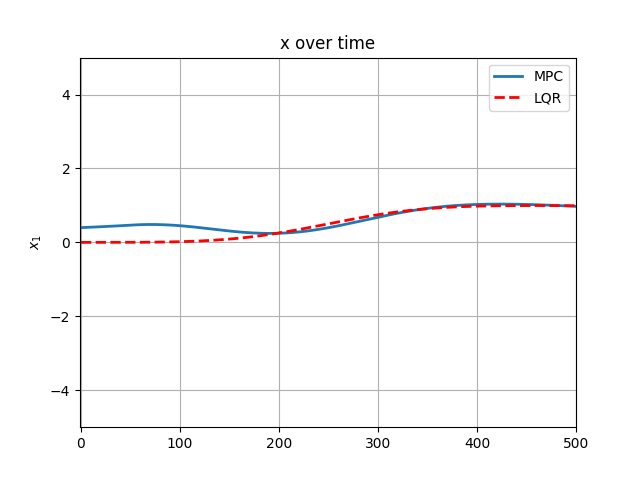
\includegraphics[width=0.9\textwidth]{pictures/mpc1.png}
\caption{$x_1$}
\label{fig:mpc1}
\end{figure}

\begin{figure}[H]
\centering
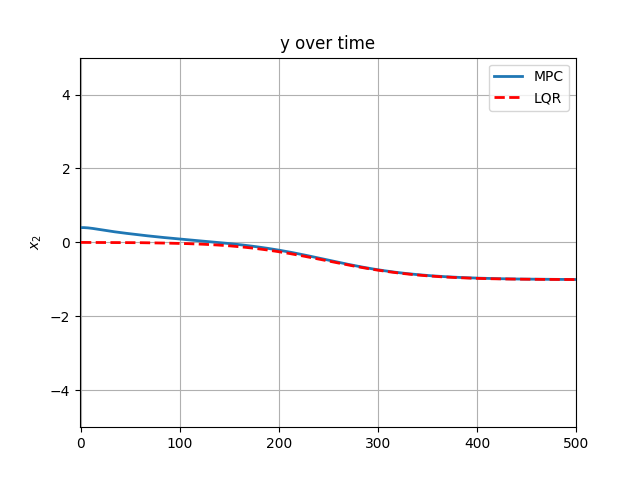
\includegraphics[width=0.9\textwidth]{pictures/mpc2.png}
\caption{$x_2$}
\label{fig:mpc2}
\end{figure}

\begin{figure}[H]
\centering
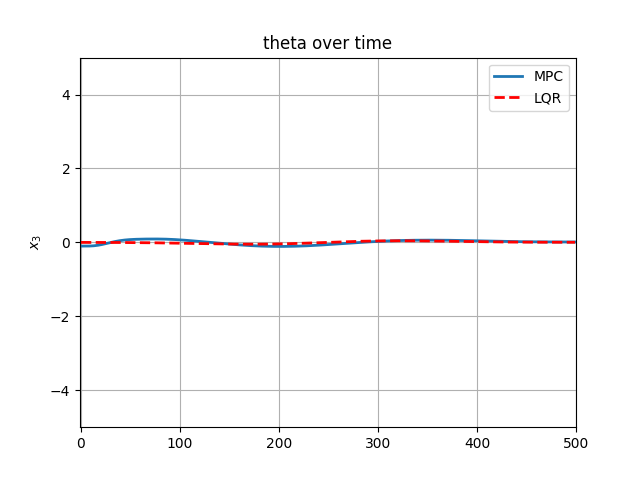
\includegraphics[width=0.9\textwidth]{pictures/mpc3.png}
\caption{$x_3$}
\label{fig:mpc3}
\end{figure}

\begin{figure}[H]
\centering
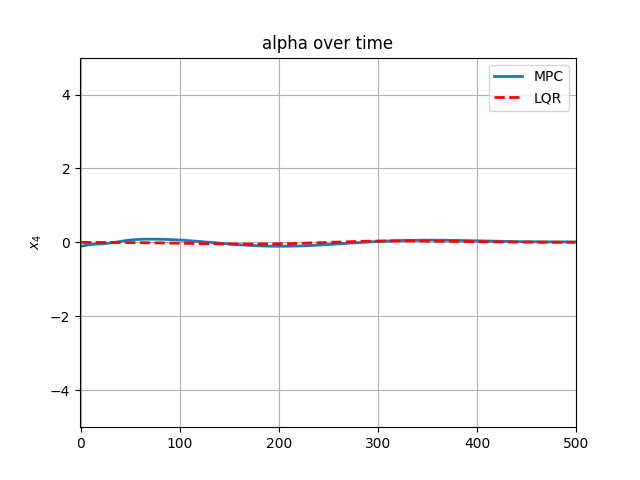
\includegraphics[width=0.9\textwidth]{pictures/mpc4.png}
\caption{$x_4$}
\label{fig:mpc4}
\end{figure}

\begin{figure}[H]
\centering
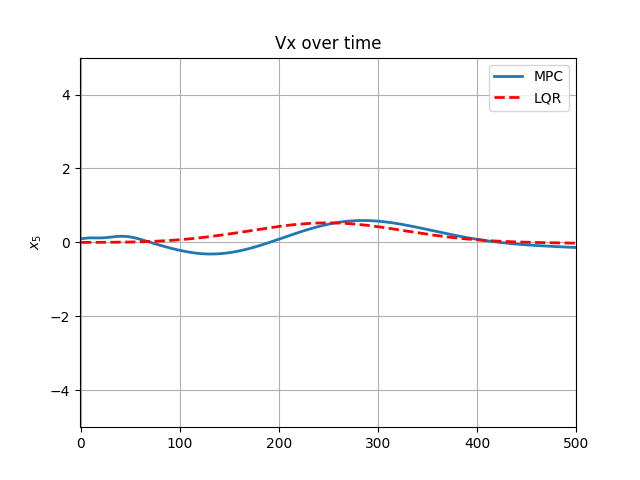
\includegraphics[width=0.9\textwidth]{pictures/mpc5.png}
\caption{$x_5$}
\label{fig:mpc5}
\end{figure}

\begin{figure}[H]
\centering
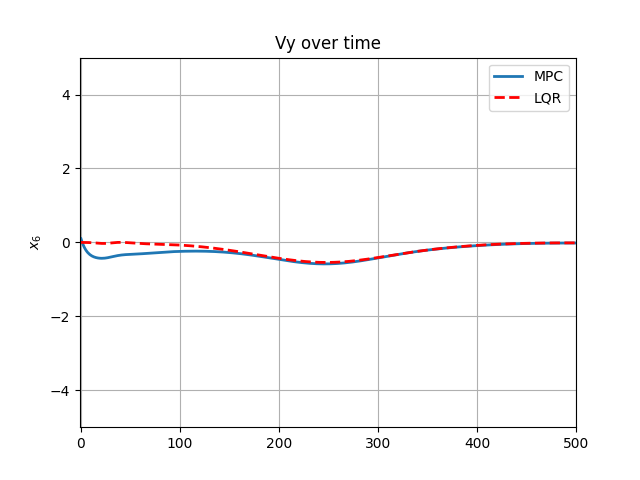
\includegraphics[width=0.9\textwidth]{pictures/mpc6.png}
\caption{$x_6$}
\label{fig:mpc6}
\end{figure}

\begin{figure}[H]
\centering
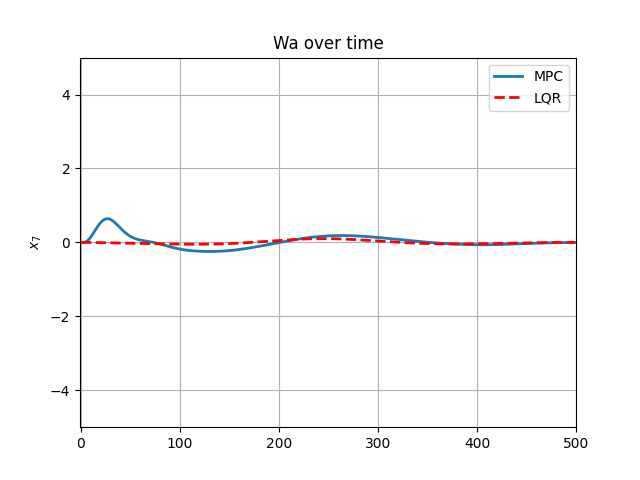
\includegraphics[width=0.9\textwidth]{pictures/mpc7.png}
\caption{$x_7$}
\label{fig:mpc7}
\end{figure}

\begin{figure}[H]
\centering
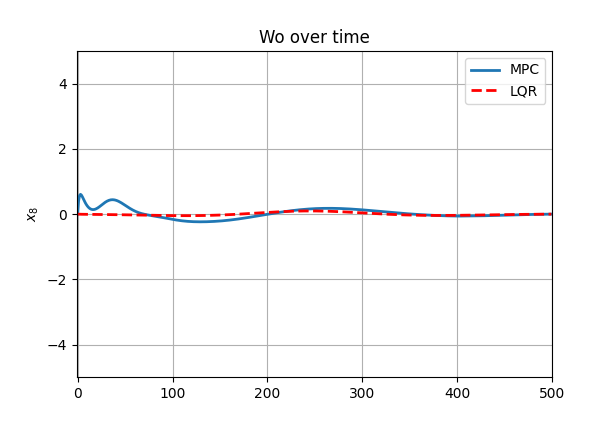
\includegraphics[width=0.9\textwidth]{pictures/mpc8.png}
\caption{$8_1$}
\label{fig:mpc8}
\end{figure}

\begin{figure}[H]
\centering
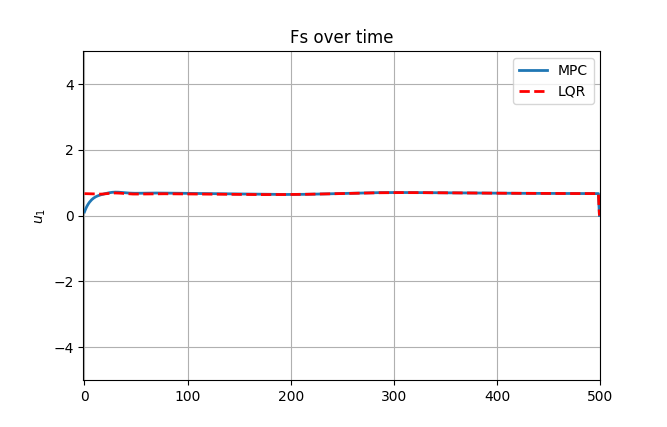
\includegraphics[width=0.9\textwidth]{pictures/mpc9.png}
\caption{$u_1$}
\label{fig:mpc9}
\end{figure}

\begin{figure}[H]
\centering
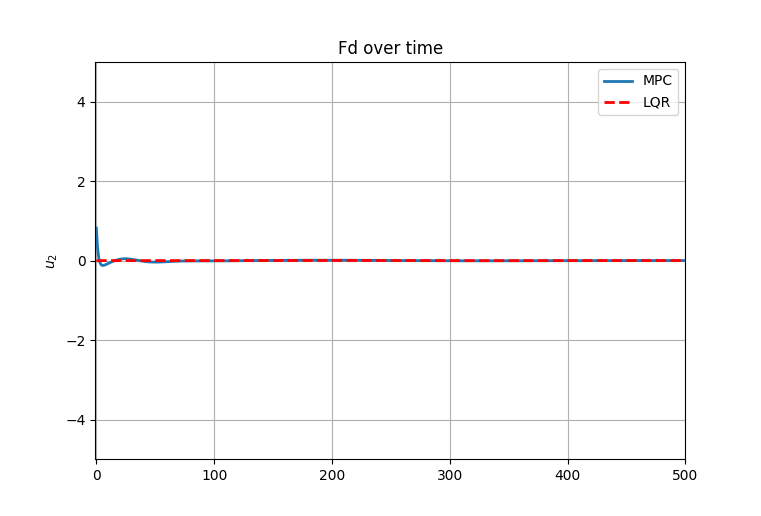
\includegraphics[width=0.9\textwidth]{pictures/mpc10.png}
\caption{$u_2$}
\label{fig:mpc10}
\end{figure}
 
\subsection{Tracking error for different initial conditions}

Given the perturbed initial condition \[ x_0 = [0.4, 0.4, -0.1, -0.1, 0.1, 0.1, 0, 0]^T\]
the following are the plots of the tracking error for single states and inputs: 


\begin{figure}[H]
\centering
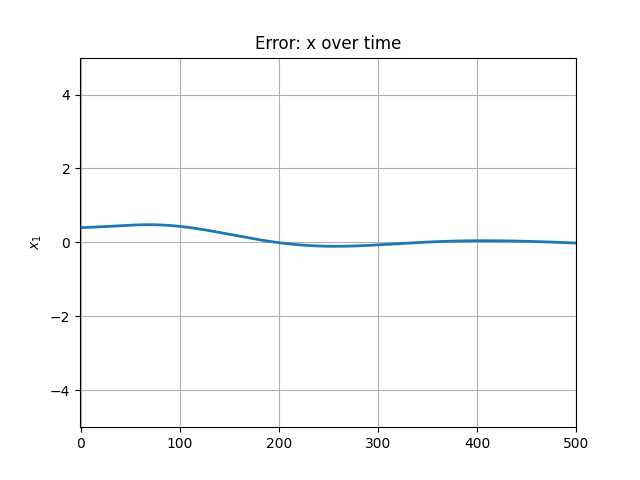
\includegraphics[width=0.83\textwidth]{pictures/mpc11.png}
\caption{Tracking error for $x_1$}
\label{fig:mpc11}
\end{figure}

\begin{figure}[H]
\centering
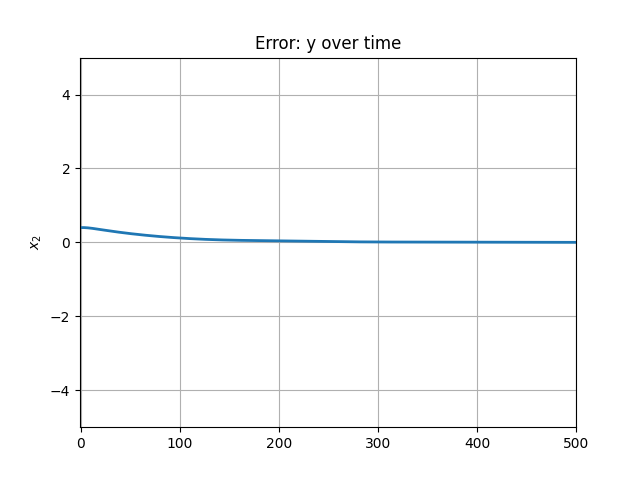
\includegraphics[width=0.9\textwidth]{pictures/mpc12.png}
\caption{Tracking error for $x_2$}
\label{fig:mpc12}
\end{figure}

\begin{figure}[H]
\centering
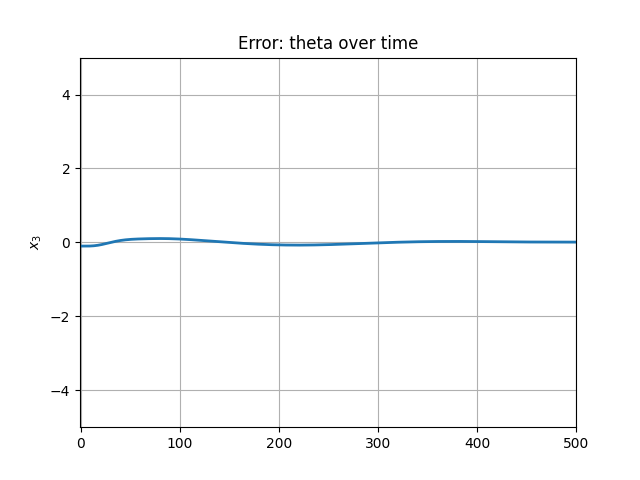
\includegraphics[width=0.9\textwidth]{pictures/mpc13.png}
\caption{Tracking error for $x_3$}
\label{fig:mpc13}
\end{figure}

\begin{figure}[H]
\centering
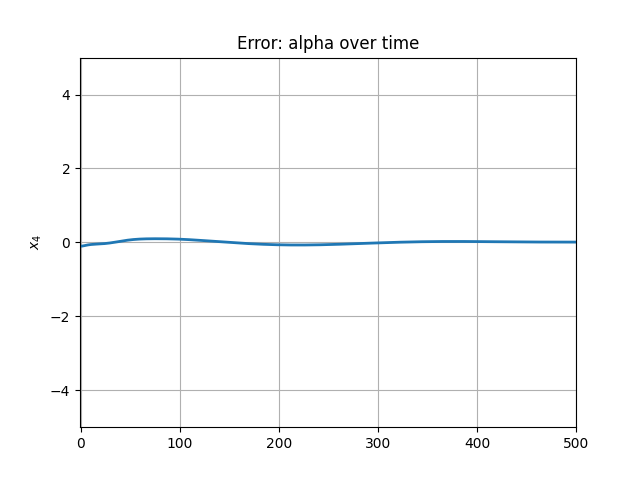
\includegraphics[width=0.9\textwidth]{pictures/mpc14.png}
\caption{Tracking error for $x_4$}
\label{fig:mpc14}
\end{figure}

\begin{figure}[H]
\centering
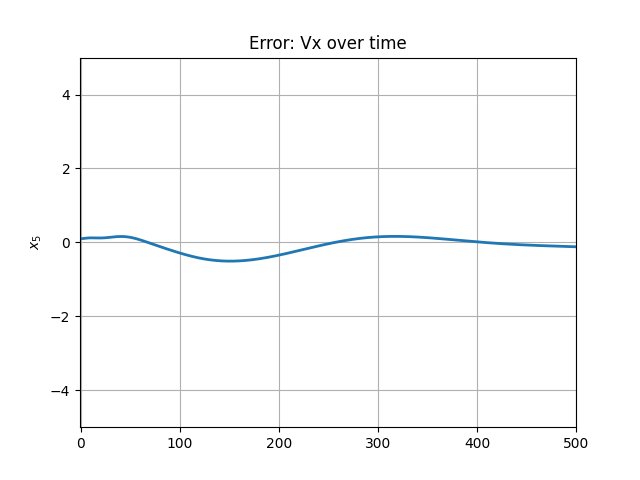
\includegraphics[width=0.9\textwidth]{pictures/mpc15.png}
\caption{Tracking error for $x_5$}
\label{fig:mpc15}
\end{figure}

\begin{figure}[H]
\centering
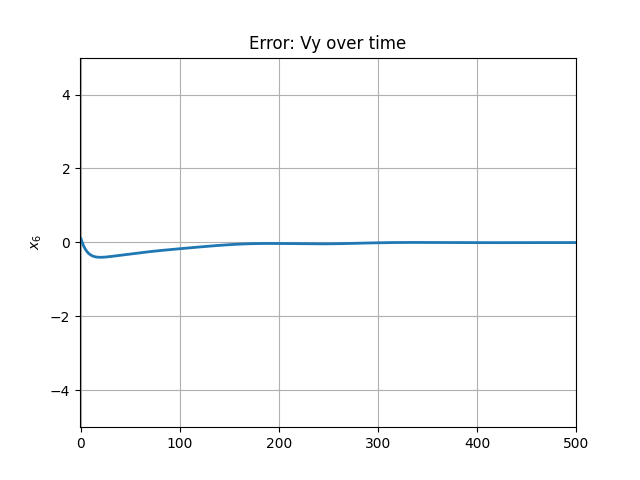
\includegraphics[width=0.9\textwidth]{pictures/mpc16.png}
\caption{Tracking error for $x_6$}
\label{fig:mpc16}
\end{figure}

\begin{figure}[H]
\centering
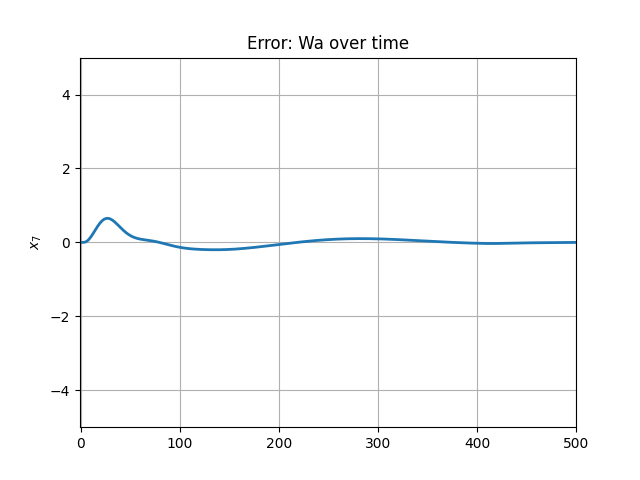
\includegraphics[width=0.9\textwidth]{pictures/mpc17.png}
\caption{Tracking error for $x_7$}
\label{fig:mpc17}
\end{figure}

\begin{figure}[H]
\centering
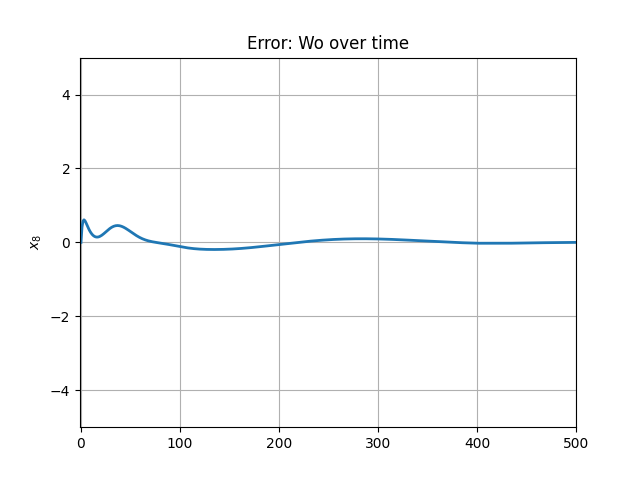
\includegraphics[width=0.9\textwidth]{pictures/mpc18.png}
\caption{Tracking error for $x_8$}
\label{fig:mpc18}
\end{figure}

\begin{figure}[H]
\centering
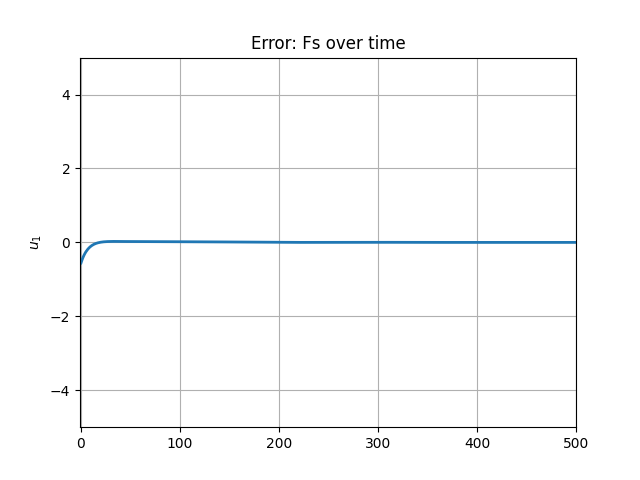
\includegraphics[width=0.9\textwidth]{pictures/mpc19.png}
\caption{Tracking error for $u_1$}
\label{fig:mpc19}
\end{figure}

\begin{figure}[H]
\centering
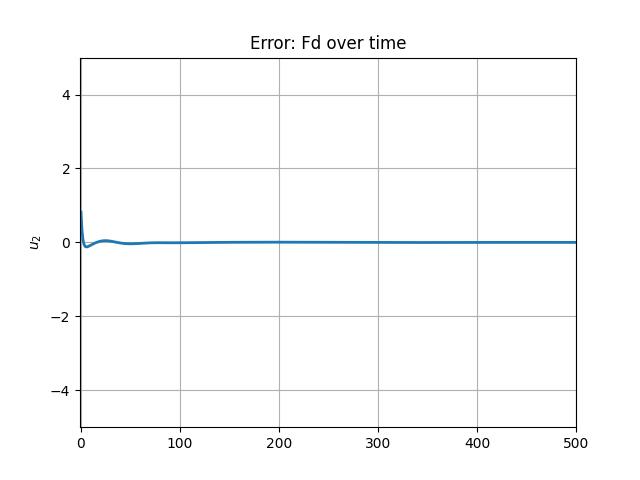
\includegraphics[width=0.9\textwidth]{pictures/mpc20.png}
\caption{Tracking error for $u_2$}
\label{fig:mpc20}
\end{figure}